\chapter{Mathematical Preliminaries}
\label{chapter:Prelims}

In this chapter, we introduce the mathematical background and notation needed to analyse model and analyse dynamic networks.

\section{Graph-Theoretic Notation}\label{section:graphNotation}

First we introduce notation for working with graphs, the central structure on which rumour spreading takes place.

\begin{definition}
	Complement Set

	\noindent
	Given a graph $G = (V, E)$, for a set of vertices $S \subseteq V$ we define the complement set $\comp{S} = V \setminus S$
\end{definition}

\begin{definition}
	Cut Set

	\noindent
	Given a graph $G = (V, E)$, for a set of vertices $S \subseteq V$ we define the cut set $ E(S, \comp{S}) = \left\{\{u, v\} \in E \mid u \in S, v \in \comp{S} \right\}.$
\end{definition}

\begin{definition}
	Degree of a vertex

	\noindent
	Given a graph $G = (V, E)$, let $d_v$ be the number of neighbouring nodes $v$ is adjacent to, i.e. $$
		d_v = |\left\{ e \in E : v \in e \right\}|
	$$
\end{definition}

\begin{definition}
	Volume of a vertex set

	\noindent
	Given a graph $G = (V, E)$ with $S \subseteq V$, let 
	$$
		\text{vol}(S) = \sum_{v \in S} d_v
	$$
\end{definition}

\begin{definition}
	Graph Isomorphism

	\noindent		
	We say two graphs $G_1 = (V_1, E_1)$ and $G_2 = (V_2, E_2)$ are isomorphic if there exists a function $f: V_1 \to V_2$ such that $\{u, v\} \in E_1$ if and only if $\{f(u), f(v)\} \in E_2$, i.e, there exists a relabelling of the nodes such that $G_1=G_2$.
\end{definition}

\section{Asymptotic Notation}

In this section, we review asymptotic notation for real valued functions. We assume the reader is familiar with this style of notation, but give precise definitions to avoid confusion. The following definitions allow us to compare functions from the natural numbers to the reals.

\begin{definition}
	$\mathcal{O}$-Notation

	\noindent
	We say $f(n) = \mathcal{O}(g(n))$ if there exists a real constant $c > 0$ and $N \in \mathbb{N}$ such that $f(n) \leq c g(n)$ for all $n \geq N$. 
\end{definition}

\begin{definition}
	$\Omega$-Notation

	\noindent
	We say $f(n) = \Omega(g(n))$ if there exists a real constant $c > 0$ and $N \in \mathbb{N}$ such that $f(n) \geq c g(n)$ for all $n \geq N$. 
\end{definition}

\begin{definition}
	$\Theta$-Notation

	\noindent
	We say $f(n) = \Theta(g(n))$ if $f(n) = \mathcal{O}(g(n))$ and $f(n) = \Omega(g(n))$
\end{definition}

\begin{definition}
	$o$-Notation

	\noindent
	We say $f(n) = o(g(n))$ if for all $c > 0$, there exists $N \in \mathbb{N}$ such that $f(n) < c g(n)$ for all $n \geq N$.
\end{definition}

\begin{definition}
	Tight

	\noindent
	If the function $f$ is bounded above by $g$ such that $f(n) = \Theta(g(n))$, then we say the bound is tight. 
\end{definition}

\begin{definition}
	Almost tight

	\noindent
	If the function $f$ is bounded above by $g$ such that $f(n) = \bigO\lb(\log n)^k g(n)\rb$ for some constant $k \geq 1$ and $g(n) = \Omega((\log n)^k)$, then we say the bound $g$ is almost tight, since for large $n$ poly-logarithmic factors become comparatively small. 
\end{definition}

\section{Discrete-time Markov Chains}

In this section we give a brief review of Markov chains and associated results needed for Section \ref{section:MEDNBound}. We assume that the reader is familiar with finite Discrete-time Markov chains, so omit the proofs in this section. For a full treatment of the subject and proofs of the theorems in this section see \cite{grimmetBook}.

\begin{definition}
	Markov Chain

	\noindent A stochastic process $\{X_n, n \geq 0 \}$ on a state space $S$ is a Markov chain if 
	$$
		\mathbb{P}(X_n = s_n | X_0 = s_0, \dots,  X_{n-1} = s_{n-1}) 
		= \mathbb{P}(X_n = s_n | X_{n-1} = s_{n-1})
	$$
	for all $n \geq 1$ and $s_0, \dots, s_n \in S$.
\end{definition}

All the Markov chains we study in this section will operate on state spaces with a finite number of elements, so henceforth all results assume that the state space is finite. For simplicity, we also restrict our study to time homogenous Markov chains, that is Markov chains $\{X_n, n \geq 0 \}$ which satisfy
$$
	\mathbb{P}(X_{n+1} = i | X_n = j)
	= \mathbb{P}(X_1 = i | X_0 = j)
$$
for all $n \geq 1$ and $i, j \in S$.

\begin{definition}
	Transition Matrix

	The transition matrix of a Markov chain $\{X_n, n \geq 0 \}$ on a state space $S$ is an $|S| \times |S|$ matrix $P=(p_{ij})_{i, j \in S}$ such that
	$$
		p_{ij} = \mathbb{P}(X_1 = j | X_0 = i)
	$$
\end{definition}

\begin{definition}
	Stationary Distribution

	\noindent
	A row vector $\pi=(\pi_i)_{i \in S}$ is a stationary distribution of a Markov chain on a state space $S$ with transition matrix $P$ if
	\begin{enumerate}
		\item $p_i \geq 0$ for all $i \in S$
		\item $\sum_{i \in S} p_i = 1$
		\item $\pi P = \pi$
	\end{enumerate}
\end{definition}

\begin{definition}
	Irreducibility

	\noindent
	A Markov chain on a state space $S$ is irreducible if for all $i, j \in S$, there exists an $n \geq 0$ such that 
	$$
		\mathbb{P}(X_n = i | X_0 = j) > 0
	$$
\end{definition}

\begin{theorem}\label{theorem:uniqueStationaryDistribution}
	An irreducible Markov chain has a unique stationary distribution.
\end{theorem}

\begin{definition}
	Period

	\noindent
	The period of state $s \in S$ in a Markov chain $\{X_n, n \geq 0 \}$ is
	$$
		\gcd\{ n \geq 1 : \mathbb{P}(X_n = s | X_0 = s)\}
	$$
	If all states have period 1, we call the Markov chain aperiodic.
\end{definition}

\begin{theorem}\label{theorem:markovChainConvergence}
	If a Markov chain is irreducible and aperiodic, then the distribution of its current state after $n$ time steps converges to its stationary distribution as $n$ tends to infinity.
\end{theorem}

Once the Markov chain has converged to the stationarity distribution we say it has reached equilibrium.

\section{Inhomogeneous Poisson Processes}\label{section:inhomoPP}

In this section we introduce a variant of the Poisson process which will be needed for Chapters \ref{chapter:AsyncUpperBound} and \ref{chapter:asyncBoundTight}. We assume the reader will be familiar with standard Poisson processes, but anticipate they may not be familiar with the inhomogeneous variant. Thus, we introduce the inhomogeneous Poisson Process from first principles.

First, a review of the fundamental structure of Poisson processes.

\begin{definition}
	Counting Process

	\noindent
	A counting process $\left\{ N(t), t \geq 0 \right\}$ is a right-continuous non-decreasing random function $N$ from non-negative reals to non-negative integers such that $N(0) = 0$.
\end{definition}

\begin{figure}[h]
	\centering
	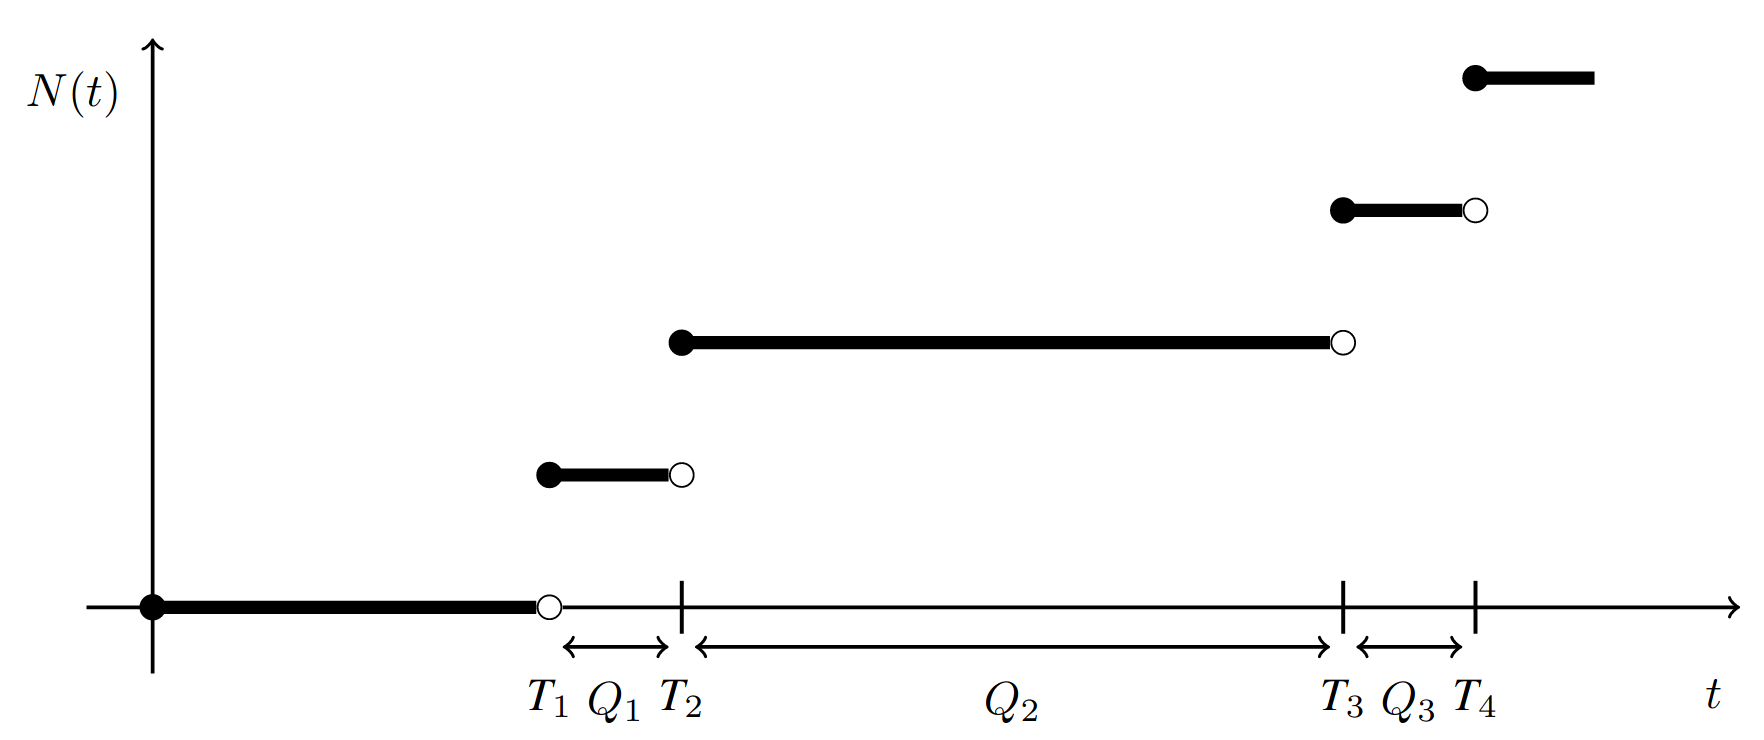
\includegraphics[width=\textwidth]{./figures/poisson_process_example.png}
	\caption{Example of a counting process from \cite{countingProcessFigure}}
	\label{fig:poissonProcessExample}
\end{figure}

We interpret the function $N$ as counting the number of occurrences of an event, where $N(t)$ represents the number of events that have occurred up to and including time $t$. We refer to the occurrences of events as `arrivals'.  Since $N$ is right-continuous, $N$ increments exactly at the times of arrivals. For example, if $a^\text{th}$ arrival happens at time $t$, then $N(t) = a$, $\lim_{x \downarrow t} = a$, and $\lim_{x \uparrow t} = a - 1$, as can be seen in Figure \ref{fig:poissonProcessExample}. Note that the number of arrivals in the interval $(s, t]$ is represented by the random variable $N(t) - N(s)$. 

Now we introduce a central definition in the theory of Poisson processes.

\begin{definition}
	Independent Increments

	A random counting process $\left\{ N(t), t \geq 0 \right\}$ has independent increments if for any $n \in \mathbb{N}$ and $0 \leq t_0 \leq t_1 \leq \dots \leq t_n \in \mathbb{R}$,
	the random variables
	$$
		N(t_1) - N(t_0), \dots, N(t_n) - N(t_{n - 1})
	$$
	are independent.
\end{definition}

We are now ready to introduce the inhomogeneous Poisson process.

\begin{definition}\label{defn:inhomoPP}
	Inhomogeneous Poisson process

	\noindent
	An inhomogeneous Poisson process ${N(t), t \geq 0}$ with rate function $\lambda(t) > 0$ is a counting process such that:
	\begin{enumerate}
		\item $N(t)$ has independent increments
		\item for all $0 \leq s \leq t$, 
		the number of arrivals in the interval $(s, t]$, 
		$N(t) - N(s)$, has a Poisson distribution with mean
		$$
			\Lambda(t) = \int_s^t \lambda(x) dx
		$$
		\item $N(0) = 0$
	\end{enumerate}
\end{definition}

Unlike the standard Poisson process, in the inhomogeneous variant, the rate of arrivals can vary over time according to the rate function $\lambda(t)$. In this report, inhomogeneous Poisson processes arise when we consider consecutive homogenous Poisson processes. We show that the cumulative arrivals of consecutive homogenous Poisson processes form an inhomogeneous Poisson process in the following theorem.

\begin{theorem}
	Let $N_1, \dots, N_m$ be independent Poisson processes, where the rate of $N_i$ is denoted by $\lambda_i$. Let $(t_1, t_2], (t_2, t_3], \dots$ be a sequence of contiguous intervals such that $t_1 = 0$ and $t_i < t_{i+1}$. Let $\{N(t), t \geq 0\}$ be a counting process such that
	$$
		N(0) = 0, \quad N(t) = N(t_i) + N_i(t - t_i)
	$$ 
	for $t \in (t_i, t_{i+1}]$ i.e, $N(t)$ counts the cumulative arrivals of consecutive homogenous Poisson processes up to time $t$. Then $N(t)$ is an inhomogeneous Poisson process with rate function $\lambda(t)$ where
	$$
		\lambda(t) = \lambda_i
	$$
	for $t \in (t_i, t_{i+1}]$.
\end{theorem}

\begin{proof}
	To prove this theorem, we verify that $N(t)$ satisfies the three conditions in Definition \ref{defn:inhomoPP}. First note that $N(t)$ has independent increments since each of the component Poisson processes are independent and have independent increments by definition. For the second condition, we analyse the distribution of the increment $N(t) - N(s)$ in two cases.

	\textbf{Case 1.} Suppose $s, t \in (t_i, t_{i+1}]$ for some $i$. 
	
	\noindent
	Then $N(t) - N(s) = N_i(t - t_i) - N_i(s - t_i)$ which has a Poisson distribution with rate $$
		\lambda_i(t-s) = \int_s^t \lambda(t)
	$$
	since $N_i$ is a Poisson process

	\textbf{Case 2.} Suppose $t \in (t_i, t_{i+1}]$ and $s \in (t_j, t_{j+1}]$ for some $i < j$.
	
	\noindent
	Note that, 
	$$
		N(t) - N(s) = (N_i(t_{i+1} - t_i) - N_i(s - t_i)) + \sum_{k=i+1}^{j-1} N_k(t_{k+1} - t_k) + N_j(t - t_j)
	$$
	Note that this is the sum of independent Poisson random variables. Hence, by the convolution of Poisson random variables we have that $N(t) - N(s)$ is a Poisson random variable with mean
	$$
		\lambda_i(t_{i+1} - s) + \sum_{k=i+1}^{j-1} \lambda_k(t_{k+1} - t_k) + \lambda_j(t - t_j) = \int_s^t \lambda(t) 
	$$
	For the third condition, note that we are given $N(0) = 0$.
\end{proof}

We now define the homogenous Poisson process in terms of the inhomogeneous process.

\begin{definition}
	(Homogeneous) Poisson process

	\noindent
	A Homogeneous Poisson process $\{N(t), t \geq 0\}$ with rate $\lambda > 0$ is a special case of the inhomogeneous Poisson process where the rate function $\lambda(t)$ is constant i.e. $\lambda(t)=\lambda > 0$ for all $t$.
\end{definition}

In this report, if we refer to the Poisson processes without qualifying whether it is homogenous our inhomogeneous, then assume the process is homogenous.

We now introduce some standard properties of the Poisson process. We omit the proofs as we assume the reader is familiar with these properties.

\begin{theorem}
	Superposition of Poisson processes

	\noindent
	Let $\{N_1(t), t \geq 0\}$ and $\{N_2(t), t \geq 0\}$ be Poisson processes with rates $\lambda_1$ and $\lambda_2$ respectively. Then $\{N_1(t) + N_2(t), t \geq 0\}$ is a Poisson process of rate $\lambda_1 + \lambda_2$.
\end{theorem}

\begin{theorem}
	Thinning of Poisson processes.

	\noindent
	Let $\{N(t), t \geq 0\}$ be a Poisson process with rate $\lambda$ and let $X_1, X_2, \dots$ be independent $\text{Bernoulli}(p)$ random variables. Let
	$$
		M(t) = \sum_{i=1}^N(t) X_i, L(t) = N(t) - M(t)
	$$
	Then $\{M(t), t \geq 0\}$ is a Poisson process of rate $p\lambda$, $\{L(t), t \geq 0\}$ is a Poisson process of rate $(1-p)\lambda$, and both processes are independent.
\end{theorem}

\section{Stochastic Domination}

In this section we introduce the idea of stochastic domination from first principles, as we anticipate this may be a new concept for some readers. We then introduce the technique of coupling, and use it to prove stochastic domination results needed for later chapters.

We start with the central definition.

\begin{definition}
	First-order Stochastic Domination

	\noindent
	Let $X$ and $Y$ be real random variables. $Y$ has a first-order stochastic dominance over $X$, denoted by $X \preceq Y$, if for all $x \in R$, 
	$$
		\mathbb{P}(Y \geq x) \geq \mathbb{P}(X \geq x)
	$$
\end{definition}

Note that not all random variables are comparable by stochastic domination, so $\preceq$ specifies a partial order between random variables. % MAYBE: Examples of r.vs that can't be related

We now consider an informal example of stochastic domination to get a better intuition for the definition.

\begin{figure}[h]
	\centering
	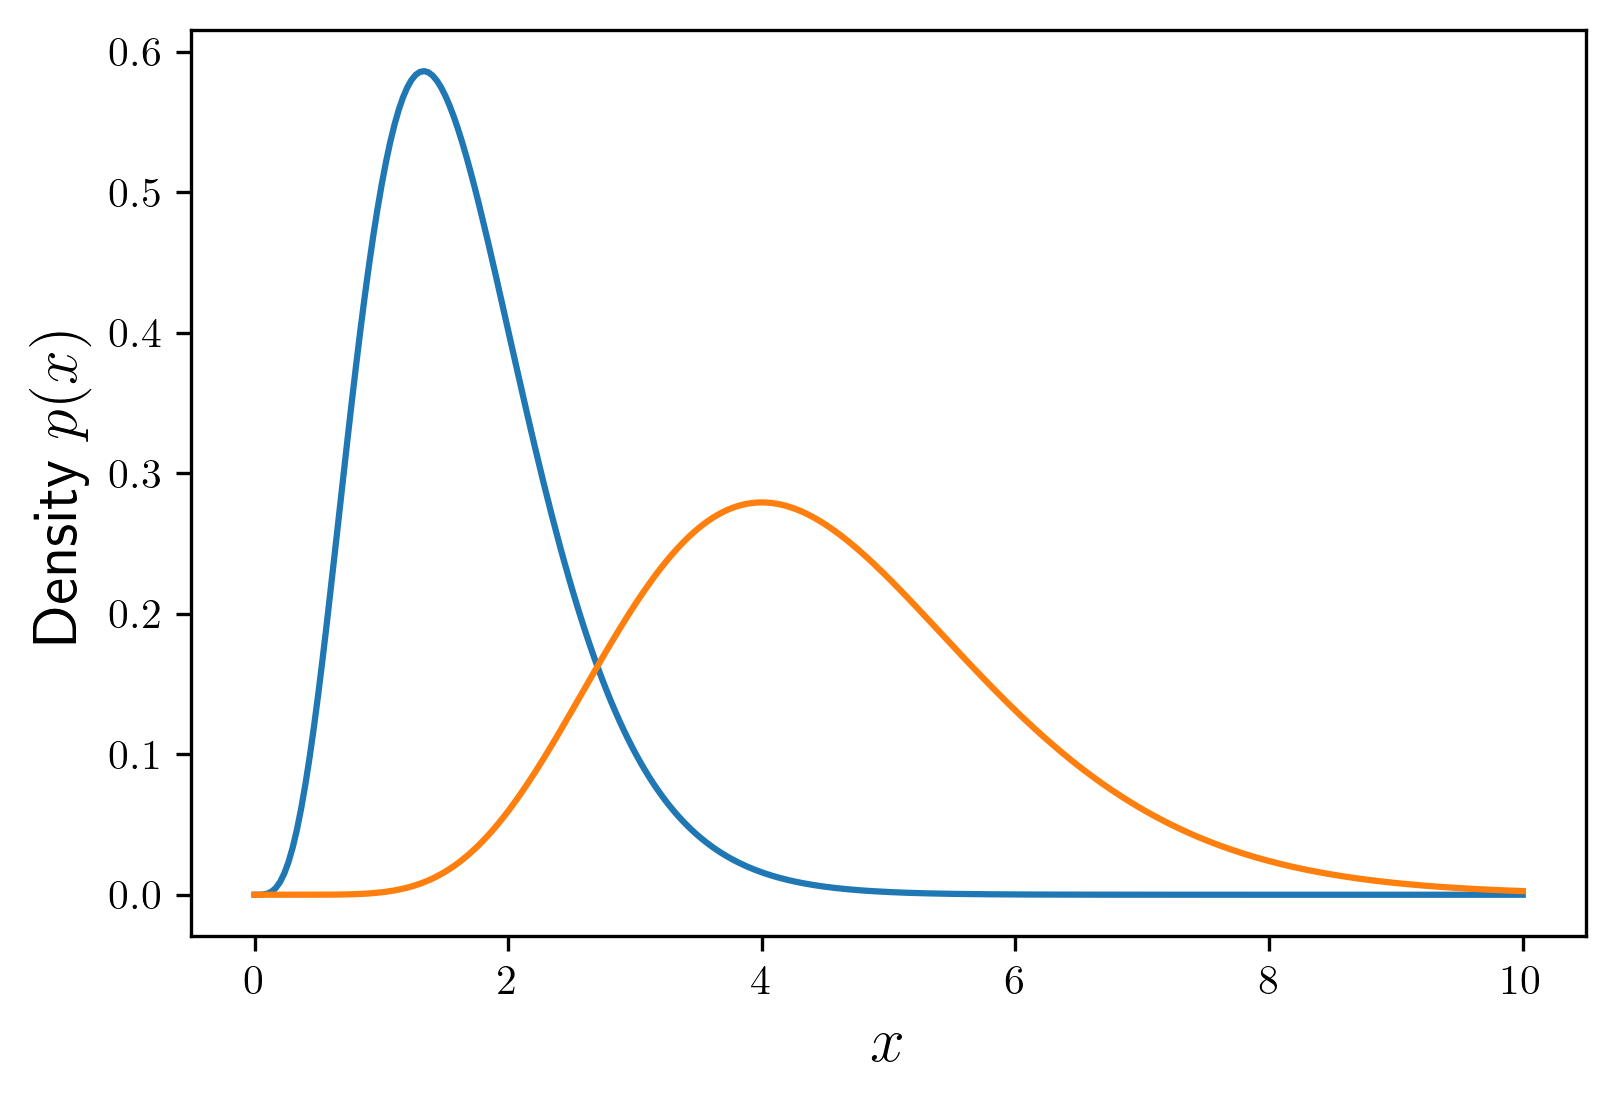
\includegraphics[width=0.8\textwidth]{./figures/stochastic_domination_pdf.png}
	\caption{Example of stochastic domination - p.d.fs}
	\label{fig:stochDomPDFs}
\end{figure}

Figure \ref{fig:stochDomPDFs} shows the probability density functions (p.d.f) of two real random variables $X$ and $Y$, where the p.d.f of $X$ is blue and the p.d.f of $Y$ is orange. In this example, $X \preceq Y$.

\begin{figure}[h]
	\centering
	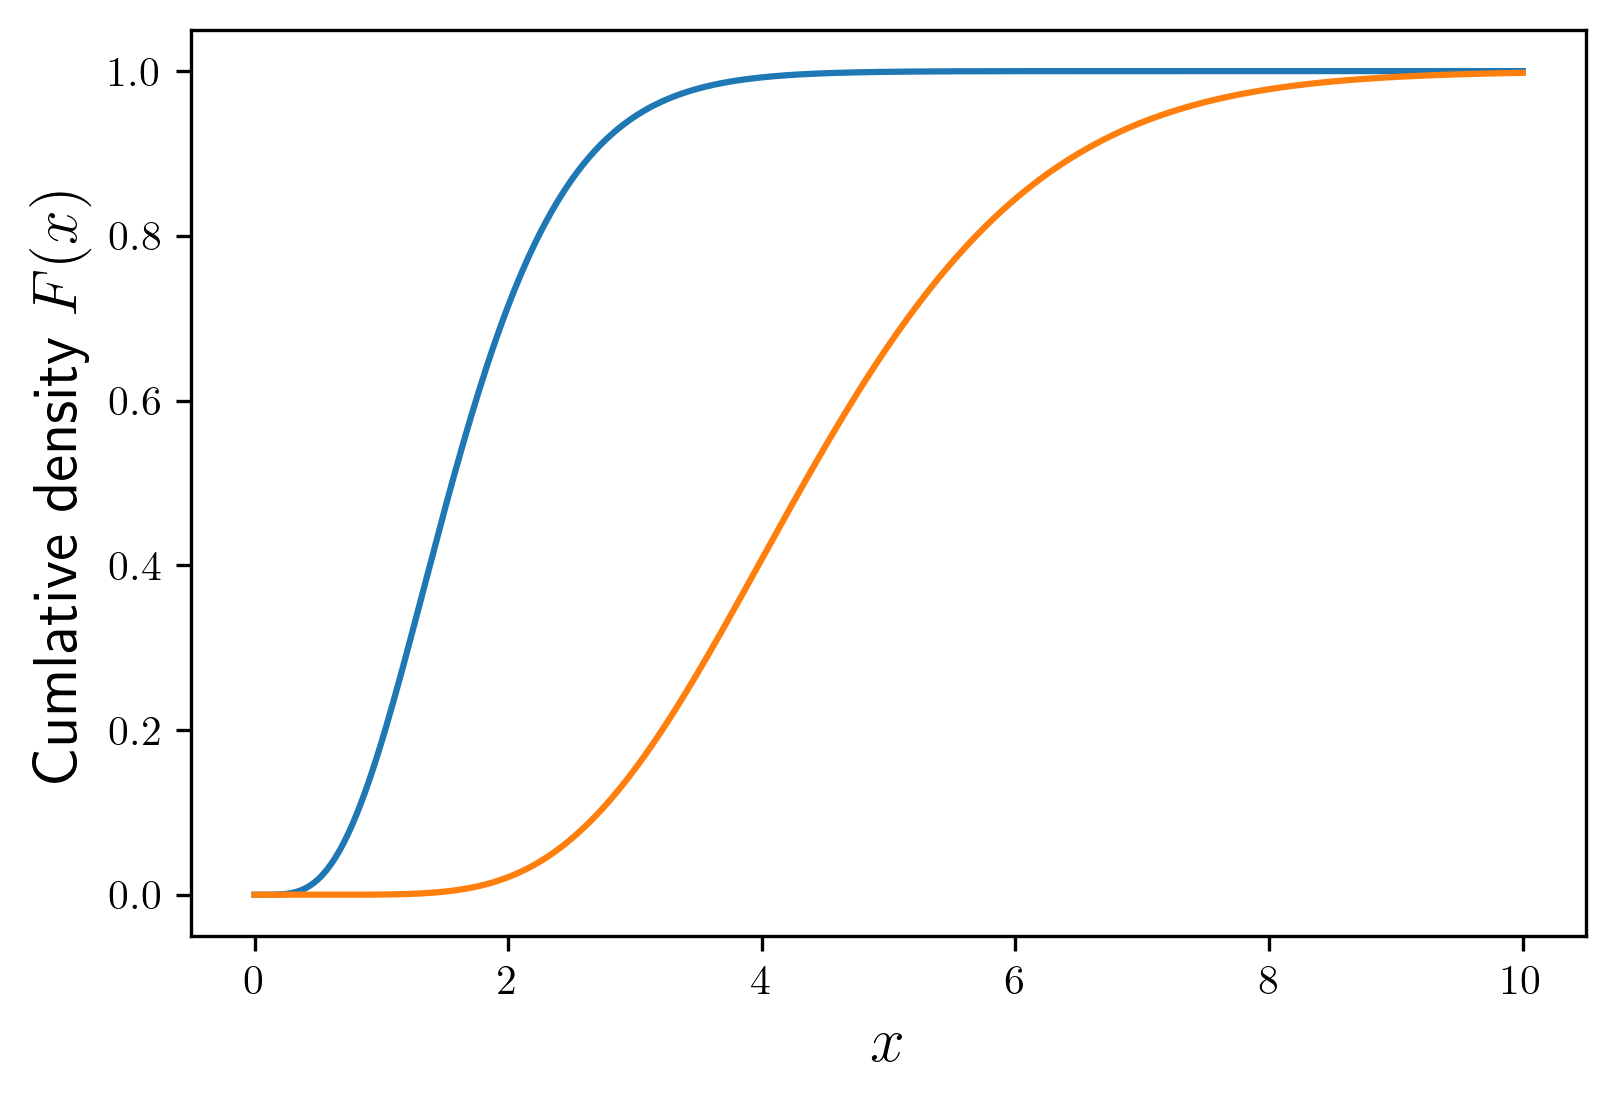
\includegraphics[width=0.8\textwidth]{./figures/stochastic_domination_cdf.png}
	\caption{Example of stochastic domination - c.d.fs}
	\label{fig:stochDomCDFs}
\end{figure}

Observe that $X \preceq Y$ if an only if $\mathbb{P}(Y \leq x) \leq \mathbb{P}(X \leq x)$. We recognise $\mathbb{P}(X \leq x)$ as the cumulative distribution function (c.d.f) of $X$. Hence, we can verify this claim by computing the cumulative  distribution functions for $X$ and $Y$, which are displayed in Figure \ref{fig:stochDomCDFs} in their associated colours. Indeed, we see that the c.d.f for $Y$ is always below the c.d.f for $X$, hence $Y$ does in fact stochastically dominate $X$.

For proofs in Chapters \ref{chapter:AsyncUpperBound} and \ref{chapter:SyncFlooding} we need to establish stochastic dominance between pairs of Binomial random variables and Poisson random variables. To do this we use a technique called coupling. First we introduce the definition of a coupling.

\begin{definition} 
	Coupling

	\noindent
	A coupling of the real random variables $X$ and $Y$ is a joint random variable $(\tilde{X}, \tilde{Y})$ such that the marginal distribution of $\tilde{X}$ is the same as $X$ (denoted $\tilde{X} \stackrel{d}{=} X$), and $\tilde{Y} \stackrel{d}{=} Y$.
\end{definition}

% MAYBE: when allowed different samples spaces, interpreation

Now we present a theorem which links couplings to first-order stochastic domination.

\begin{theorem}\label{theorem:couplingDomination}
	The real random variable $X$ is stochastically dominated by the real random variable $Y$ if and only if there exists a coupling $(\tilde{X}, \tilde{Y})$ of $X$ and $Y$ such that
	$$
		\mathbb{P}(\tilde{Y} \geq \tilde{X}) = 1
	$$
\end{theorem}

\begin{proof}
	We prove the forwards implication. Suppose there exists a coupling $(\tilde{X}, \tilde{Y})$ of $X$ and $Y$ such that $\mathbb{P}(\tilde{Y} \geq \tilde{X}) = 1$. Then for all $x \in \mathbb{R}$
	\begin{align*}
		\mathbb{P}(X \geq x) &= \mathbb{P}(\tilde{X} \geq x) & \text{since } \tilde{X} \stackrel{d}{=} X \\
		&\leq \mathbb{P}(\tilde{Y} \geq x) & \text{since with probability 1, } \tilde{Y} \geq \tilde{X} \\
		&= \mathbb{P}(Y \geq x) & \text{since } \tilde{Y} \stackrel{d}{=} Y 
	\end{align*}

	We omit the proof for the reverse implication as we only use the forwards implication. For the proof of the reverse implication, see \cite{coupling}.
\end{proof}

Using Theorem \ref{theorem:couplingDomination}, we can establish stochastic domination between random variables by finding a coupling. We first show this technique	for pairs of Poisson random variables

\begin{theorem}\label{theorem:poissonDomination}
	Let $0 < \lambda < \mu$. If $X \sim \text{Poisson}(\lambda)$ and $Y \sim \text{Poisson}(\mu)$ are independent random variables, then $X \preceq Y$. 
\end{theorem}

\begin{proof}
	Let $\tilde{X} \sim \text{Poisson}(\lambda)$, $\tilde{Z} \sim \text{Poisson}(\mu - \lambda)$ be independent random variables. Take $\tilde{Y} := \tilde{X} + \tilde{Z}$. Since $\tilde{X}$ and $\tilde{Z}$ are independent, we have that $\tilde{Y} \sim \text{Poisson}(\mu)$ by the convolution of Poisson random variables. Thus, as $\tilde{X} \stackrel{d}{=} X$ and $\tilde{Y} \stackrel{d}{=} Y $, we have established a coupling $(\tilde{X}, \tilde{Y})$ for $X$ and $Y$. Note that since $\tilde{Z} \geq 0$, the value taken by $\tilde{Y}$ is always at least the value taken by $\tilde{X}$. Since we have found a coupling $(\tilde{X}, \tilde{Y})$ of $X$ and $Y$ where $\mathbb{P}(\tilde{Y} \geq \tilde{X}) = 1$, by Theorem \ref{theorem:couplingDomination}, $X \preceq Y$.
\end{proof}

Now we use coupling to establish first-order stochastic dominance between pairs of Binomial random variables.

\begin{theorem}\label{theorem:binomialDomination}
	Let $X \sim \text{Binomial}(n_1, p)$ and $Y \sim \text{Binomial}(n_2, p)$ be independent random variables with $n_1 < n_2$. Then $X$ is stochastically dominated by $Y$.
\end{theorem}

\begin{proof}
	Let $X_1, \dots, X_{n_2}$ be a sequence of independent Bernoulli random variables where $\mathbb{P}(X_i = 1) = p$. We observe that $\tilde{X} := \sum_{i=1}^{n_1} X_i \sim \text{Binomial}(n_1, p)$ and $\tilde{Y} := \sum_{i=1}^{n_2} X_i \sim \text{Binomial}(n_2, p)$. Since $X_i \geq 0$ for all $i$, and $\tilde{Y} = \tilde{X} + X_{n_1 + 1} + \dots + X_{n_2}$, we have that $\tilde{X} \leq \tilde{Y}$. Hence, by Theorem \ref{theorem:couplingDomination}, $X \preceq Y$.
\end{proof}
